\chapter{[简洁] openpyxl库}
\label{sec:openpyxl库}
\codeinline{openpyxl} 是一个用于读取、写入和修改 Excel 文件的库，它支持 \codeinline{xlsx} 格式的文件,不用再担心格式问题。

相较于 \codeinline{xlrd} 和 \codeinline{xlwt}，\codeinline{openpyxl} 更加强大，支持更多的功能，例如合并单元格、设置单元格样式、添加图表等。

\codeinline{openpyxl}唯一的缺点就是对Excel中VBA(Visual Basic Applications)支持的并不友好。

\section{安装}
\label{subsec:openpyxl安装}
\begin{lstlisting}[style=demostyle,numbers=none]
# pip 安装
pip install openpyxl

# conda 安装
conda install openpyxl
\end{lstlisting}

\section{创建Excel文件}
\begin{lstlisting}[style=demostyle,numbers=none]
from openpyxl import Workbook

# 创建一个新的工作簿
wb = Workbook()

# 保存工作簿到文件
wb.save("new_excel_file.xlsx")
\end{lstlisting}

\section{读取Excel内容}
\label{subsec:openpyxl读取Excel内容}
需要注意，openpyxl与xlrd、xlwt不同，
cell方法中的row、column参数从1开始， 
即工作表中的行号、列号与Excel工作表一样，都以1作为起始坐标，
而xlrd、xlwt却以0作为起始坐标。

\subsection{load\_workbook() 打开文件}
\begin{lstlisting}[style=demostyle,numbers=none]
from openpyxl import load_workbook    
# 打开一个Excel文件
wb = load_workbook('excel/example.xlsx')
\end{lstlisting}

\subsection{sheet表单}
针对Excel文件中的sheet表单，openpyxl提供了以下几个方法：
\begin{enumerate}[label=\arabic*)]
    \item \codeinline{get\_sheet\_names()}：获取工作簿中所有的sheet名称
    \item \codeinline{get\_sheet\_by\_name()}：根据名字获取sheet
    \item \codeinline{get\_sheet\_by\_index()}：根据索引获取sheet
\end{enumerate}

\begin{lstlisting}[style=demostyle,numbers=none]
## max_row 获取最大行数
## max_column 获取最大列数
## cell() 获取单元格
## cell().value 获取单元格的值
\end{lstlisting}



\begin{lstlisting}[style=pythonstyle,numbers=left]
from openpyxl import load_workbook

# 1. 打开一个Excel文件
workbook = load_workbook('excel/example.xlsx')

# 2. 获取工作簿中所有的sheet名称
sheet_names = workbook.sheetnames
print(f"Sheet names: {sheet_names}")

# 3. 根据名字获取sheet
sheet_by_name = workbook[sheet_names[0]]
print(f"Sheet by name: {sheet_by_name.title}")

# 4. 根据索引获取sheet (openpyxl没有直接根据索引获取sheet的方法，我们通过sheetnames间接获取)
sheet_by_index = workbook[sheet_names[1]]
print(f"Sheet by index: {sheet_by_index.title}")

# 5. 获取最大行数和最大列数
max_row = sheet_by_name.max_row
max_column = sheet_by_name.max_column
print(f"Max row: {max_row}, Max column: {max_column}")

# 6. 获取特定单元格
cell = sheet_by_name.cell(row=1, column=1)
print(f"Cell at (1, 1): {cell}")

# 7. 获取单元格的值
cell_value = cell.value
print(f"Value of cell at (1, 1): {cell_value}")

# 打印所有单元格值的示例
for row in sheet_by_name.iter_rows(min_row=1, max_row=max_row, min_col=1, max_col=max_column):
    for cell in row:
        print(f"Row {cell.row}, Column {cell.column}: {cell.value}")
\end{lstlisting}

\begin{lstlisting}[style=demostyle,numbers=none]
Sheet names: ['教师', '学生', 'Sheet3']
Sheet by name: 教师
Sheet by index: 学生
Max row: 2, Max column: 3
Cell at (1, 1): <Cell '教师'.A1>
Value of cell at (1, 1): 姓名
Row 1, Column 1: 姓名
Row 1, Column 2: 性别
Row 1, Column 3: 学号
Row 2, Column 1: 贾继伟
Row 2, Column 2: 男
Row 2, Column 3: 20233120098
\end{lstlisting}

\section{写入Excel内容}
\label{subsec:openpyxl写入Excel内容}
\codeinline{openpyxl}除可以创建新工作簿来写数据外，还可以修改已存在的工作簿，该过程不再需要使用\codeinline{xlutils}库。

\begin{lstlisting}[style=demostyle,numbers=none]
# openpyxl 的函数
## Workbook() 创建一个新的工作簿
## create_sheet() 创建一个新的工作表
## save() 保存工作簿
## append() 添加数据
## merge_cells() 合并单元格
## unmerge_cells() 取消合并单元格
\end{lstlisting}

\begin{lstlisting}[style=pythonstyle,numbers=left]
from openpyxl import Workbook

# 1. 创建一个新的工作簿
workbook = Workbook()

# 2. 创建一个新的工作表
sheet = workbook.active
sheet.title = 'NewSheet1'  # 修改工作表的标题
print(f"Created new sheet with title: {sheet.title}")

# 3. 添加数据到工作表
data = [
    ["Name", "Age", "City"],
    ["Alice", 30, "New York"],
    ["Bob", 25, "Los Angeles"],
    ["Charlie", 35, "Chicago"]
]

for row in data:
    sheet.append(row)

# 4. 合并和取消合并单元格
# 合并单元格
sheet.merge_cells('A1:C1')
print("Merged cells A1 to C1")
sheet.merge_cells('A2:C2')
print("Merged cells A2 to C2")

# 保存之前取消合并单元格
sheet.unmerge_cells('A1:C1')
print("Unmerged cells A1 to C1")

# 5.在添加一个工作表
new_sheet = workbook.create_sheet(title='AnotherSheet')
print(f"Created another sheet with title: {new_sheet.title}")

new_sheet['A1'] = 'This is another sheet'
new_sheet.cell(row=2, column=1).value='贾继位'

# 5.保存工作簿                                                            
workbook.save('new_workbook.xlsx')
print("Workbook saved as new_workbook.xlsx")
\end{lstlisting}

\begin{figure}[htpb]
        \centering
        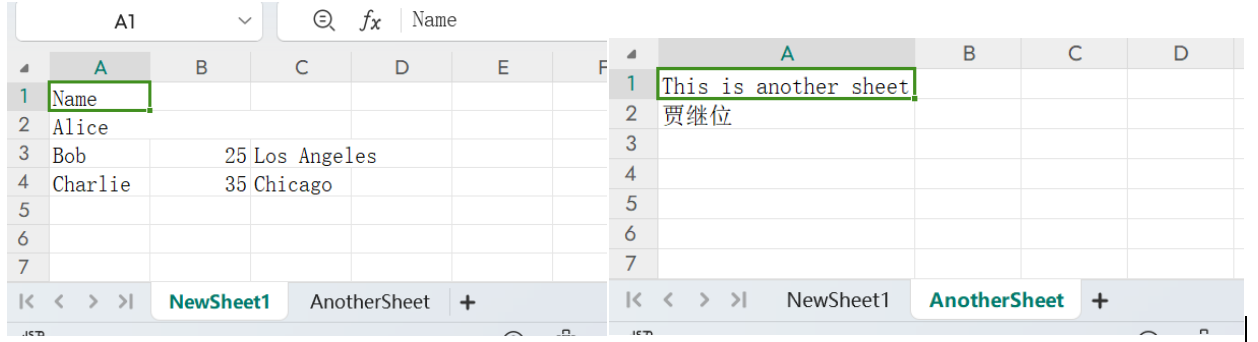
\includegraphics[width=0.8\textwidth]{part/自动化/办公自动化/pic/excel/openpyxl写入、合并演示.png}
        \caption{openpyxl写入、合并演示}
        \label{fig:openpyxl写入、合并演示}
\end{figure}


\section{修改Excel文件单元格内容}
\label{subsec:openpyxl修改现有的Excel文件}
如果想修改已存在的工作簿，只需将创建工作簿的\codeinline{openpyxl.Workbook()}方法替换为\codeinline{openpyxl.load\_workbook()}方法即可。

\section{修改Excel文件样式}
\label{subsec:openpyxl修改Excel文件样式}
\codeinline{openpyxl}支持设置单元格的样式，例如字体、颜色、对齐方式等。

主要分为以下几个部分:
\begin{enumerate}[label=\arabic*)]
    \item Font: 字体样式
    \item PatternFill: 填充样式
    \item Border: 边框样式
    \item Alignment: 对齐样式
\end{enumerate}

\subsection{基本样式}
\label{subsubsec:openpyxl基本样式}
\begin{lstlisting}[style=demostyle,numbers=none]
# openpyxl 的函数
## Font() 创建字体样式
## PatternFill() 创建填充样式
## Border() 创建边框样式
## Side() 创建边框样式
## Alignment() 创建对齐样式
## NamedStyle() 创建命名样式
## Style() 创建样式
\end{lstlisting}

\begin{lstlisting}[style=pythonstyle,numbers=left]
from openpyxl import Workbook
from openpyxl.styles import Font, PatternFill, Border, Side, Alignment

# 1. 创建一个新的工作簿和工作表
workbook = Workbook()
sheet = workbook.active
sheet.title = "StyledSheet"

# 2. 定义字体样式
font = Font(name='Arial', size=14, bold=True, italic=False, color='FF0000')
# 其中颜色也可以这样写 color=colors.RED

# 3. 定义不同的PatternFill效果
fill_types = [
    'solid', 'lightVertical', 'lightGray', 'gray0625', 'darkGray', 'gray125',
    'lightDown', 'lightHorizontal', 'darkDown', 'lightUp', 'lightTrellis', 'darkGrid',
    'darkTrellis', 'lightGrid', 'darkVertical', 'darkHorizontal', 'mediumGray', 'darkUp'
]

# 4. 定义边框样式和不同颜色
border_colors = ['FF0000', '00FF00', '0000FF', 'FFFF00', 'FF00FF', '00FFFF']
border_styles = [Border(
    left=Side(style='thin', color=color),
    right=Side(style='thin', color=color),
    top=Side(style='thin', color=color),
    bottom=Side(style='thin', color=color)
) for color in border_colors]

# 5. 定义对齐样式
alignment = Alignment(horizontal='center', vertical='center')

# 6. 将不同的PatternFill效果应用到不同单元格
for i, fill_type in enumerate(fill_types):
    print(f"Applying {fill_type} fill")
    fill = PatternFill(fill_type=fill_type, start_color='FFFF00', end_color='FFFF00')
    cell = sheet.cell(row=i + 1, column=1, value=f"{fill_type} fill")
    cell.font = font
    cell.fill = fill
    cell.border = border_styles[i % len(border_styles)]
    cell.alignment = alignment

# 7.设置行高和列宽
sheet.row_dimensions[1].height = 30 # 设置第一行的行高为30
sheet.column_dimensions['A'].width = 20 # 设置第一列的列宽为20

# 8. 保存工作簿    
workbook.save('styled_workbook_complete.xlsx')
print("Workbook saved as styled_workbook_complete.xlsx")
\end{lstlisting}

\begin{figure}[htpb]
        \centering
        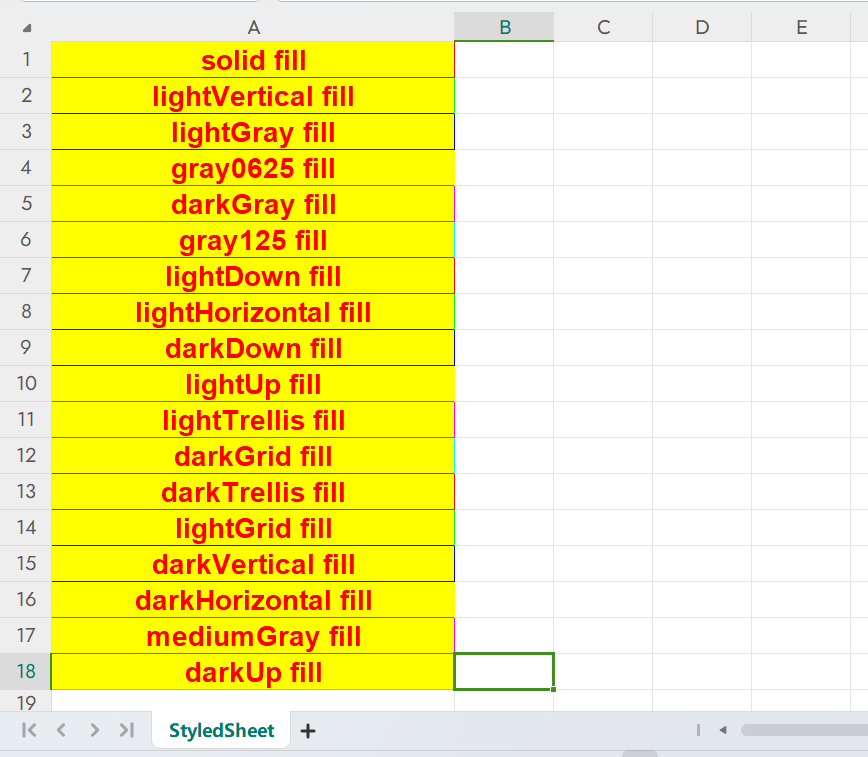
\includegraphics[width=0.8\textwidth]{part/自动化/办公自动化/pic/excel/openpyxl修改样式效果.png}
        \caption{openpyxl修改样式效果}
        \label{fig:openpyxl修改样式效果}
\end{figure}

\subsection{自定义样式}
\label{subsubsec:openpyxl自定义样式}
\begin{lstlisting}[style=pythonstyle,numbers=none]
from openpyxl import Workbook
from openpyxl.styles import Font, PatternFill, Border, Side, Alignment, NamedStyle

# 1. 创建一个新的工作簿和工作表
workbook = Workbook()
sheet = workbook.active
sheet.title = "StyledSheet"

# 2. 创建字体样式
font = Font(name='Arial', size=14, bold=True, italic=False, color='FF0000')

# 3. 创建填充样式
fill = PatternFill(fill_type='solid', start_color='FFFF00', end_color='FFFF00')

# 4. 创建边框样式
side = Side(style='thin', color='000000')
border = Border(left=side, right=side, top=side, bottom=side)

# 5. 创建对齐样式
alignment = Alignment(horizontal='center', vertical='center')

# 6. 将这些样式应用到特定单元格
cell = sheet.cell(row=1, column=1, value="Styled Text")
cell.font = font
cell.fill = fill
cell.border = border
cell.alignment = alignment

# 7. 创建命名样式
named_style = NamedStyle(name="highlight")
named_style.font = Font(name='Arial', size=12, bold=True, color='FFFFFF')
named_style.fill = PatternFill(fill_type='solid', start_color='FF5733')
named_style.border = Border(left=Side(style='thin', color='FF5733'),
                            right=Side(style='thin', color='FF5733'),
                            top=Side(style='thin', color='FF5733'),
                            bottom=Side(style='thin', color='FF5733'))
named_style.alignment = Alignment(horizontal='center', vertical='center')

# 注册命名样式
workbook.add_named_style(named_style)

# 应用命名样式到特定单元格
cell2 = sheet.cell(row=2, column=1, value="Named Style")
cell2.style = named_style

# 8. 保存工作簿
workbook.save('styled_workbook_complete.xlsx')
print("Workbook saved as styled_workbook_complete.xlsx")
\end{lstlisting}

\begin{figure}[htpb]
        \centering
        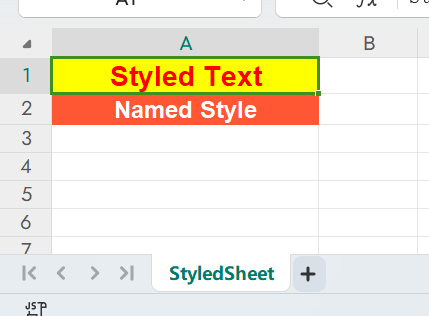
\includegraphics[width=0.8\textwidth]{part/自动化/办公自动化/pic/excel/openpyxl自定义样式效果.png}
        \caption{openpyxl自定义样式效果}
        \label{fig:openpyxl自定义样式效果}
\end{figure}

\section{操作大型Excel文件}
\label{subsec:openpyxl操作大型Excel文件}
当要处理大型工作簿时，直接将整个工作簿载人程序的操作是不合理的，数据量过大
会占用过多内存，从而影响程序本身的运行速度，导致程序出现“卡顿”、闪退等情况。

\codeinline{openpyxl}提供了一种更加高效的方式来处理大型工作簿，即使用\codeinline{read\_only}模式和\codeinline{write\_only}模式。

\begin{enumerate}[label=\arabic*)]
    \item 在\codeinline{read\_only}模式：

        openpyxl可以使用恒定的内存来处理无限的数据，其原理就是先处理一部分数据，处理完后，释放占用的内存，然后继续读入部分数据进行处理。这种方式可以快速读取大型工作簿中的数据。但需要注意，在该模式下，不允许对工作表进行写操作。

    \item 在\codeinline{write\_only}模式：

        openpyxl也是通过类似的原理将大量数据分批写入工作簿中的0
不同之处在于，该模式下不允许对工作表进行读操作。
\end{enumerate}

\subsection{read\_only模式}
\label{subsubsec:openpyxlread_only模式}
使用openpyxl的read only模式非常简单，只需在使用load\_workbook方法时将read only参数设置为True即可

\begin{lstlisting}[style=pythonstyle,numbers=left]
from openpyxl import load_workbook

# 在read_only模式下载入大型工作簿
wb = load_workbook('excel/large_workbook.xlsx', read_only=True)
# 选择 big_sheet1 工作表
sheet = workbook['big_sheet1']

for row in wb.iter_rows:  # 逐行读取数据
    for cell in row:      # 逐列读取数据
        print(cell.value)
\end{lstlisting}

\subsection{write\_only模式}
\label{subsubsec:openpyxlwrite_only模式}
使用openpyxl的write only模式也非常简单，只需在使用load\_workbook方法时将write only参数设置为True即可

\begin{lstlisting}[style=pythonstyle,numbers=left]
from openpyxl import Workbook
from openpyxl.cell import WriteOnlyCell
from openpyxl.comments import Comment
from openpyxl.styles import Font

# write_only 设置为 True
wb = Workbook(write_only=True)

# write_only模式下不会包含任何工作表，需要使用create_sheet方法自行仓U建
ws = wb.create_sheet()

# write_on1y模式下，单元格想要具有样式，就只能使用WriteOnlyCell创建单元格
cell = WriteOnlyCell (ws, 状态写入的内容')

# 为单元格设置字体样式
cell. font = Font (name='微软雅黑', size=36)

# 插入Excel批注
cell. comment = Comment (text='这是一个批注'，author='贾继伟')

# write_on1y模式下只能使用append方法添力口数据
## 在write_only模式下，不可在任意位置使用cell 或 iter_rows方法，
## 在添加数据时只能使用append方法
ws.append([cell, 2.333, None])

# 保存
wb save('write_only.xlsx')
\end{lstlisting}